\documentclass[twoside,single]{lion-msc}

\title{Electrochemically changing potential}
\author{Sebastiaan Van Mulken}
\studentid{0950815}
\supervisor{Biswajit Pradhan \\ \hspace*{\fill}Michel Orrit}
\corrector{To be determined}

\begin{document}
\maketitle

\chapter{Results and discussion}

The experiments were performed with the blue copper protein azurin from Pseudomonas aeruginosa, labeled with ATTO655 (refered to as CuAz in the rest of the analysis). This small protein, with a molecular mass of 14 kDa, is involved in electron transfer (ET) reactions in a variety of both plants and bacteria. Its label, ATTO655, has been chosen since its properties have been well documented \ref{Zhu2011}. The labeling site used in this experiment is K122 (lysine at position 122), one of the closest labeling sites to the copper center of CuAz. In the future one could label ATTO655 to a labeling site further from the copper so that the inner-dye distance changes from less to greater than the F\"{o}rster radius $R_{0}$ value for maximal sensitivity \cite{Roy2008}. 
Beside the blue copper protein azurin, zinc azurin (ZnAz) was also used to perform experiments. However, for simplicity, current knowledge and time restraints, only the blue copper protein will be discussed.

\section*{Data collection} \label{data_coll}
The sample, mounted on the scanning stages, was brought into the focal plane of the objective. To find the wire on the surface, images of (80 x 80) ($\upmu \textup{m}^{2}$) were recorded as x-y scans. Once the wire was located, a positive and negative potential is applied and captured to detect the blinking CuAz. Images of typically (20 x 20) ($\upmu \textup{m}^{2}$) were recorded in which at least 10 blinking molecules were present. To collect data from a single molecule, the laser was parked on the blinking molecule and measurements were made for 60 seconds. Once all the blinking molecules of interest were measured, a new potential was applied and this process repeated. Many fluorophores bleach within seconds, thus only the time traces of those molecules who survived all the different potentials were included for further analysis. 

To make sure that the surroundings of the singe molecules were indeed the intended potential, the I-t curves were recorded at the same time.


\section*{Time trace analysis}
The software used for the fluorescence lifetime imaging and correlation software is SymPhoTime 64. With the help of this program, timetraces and its specific parameters are saved in .pt3 files. Older versions of SymPhoTime saved this data into .t3r files. Previous PhD student .. had written a program in MATLAB R2012b and C++ to read out the .t3r files and transfer the timetraces into multiple .dat files. This program has been adjusted in such a way it can read out the .pt3 files from the newer version of SymPhoTime 64. It allows you to manually select parts of the timetrace, as is shown in Figure \ref{timetrace_selection}.

\begin{figure}[ht!]
\centering
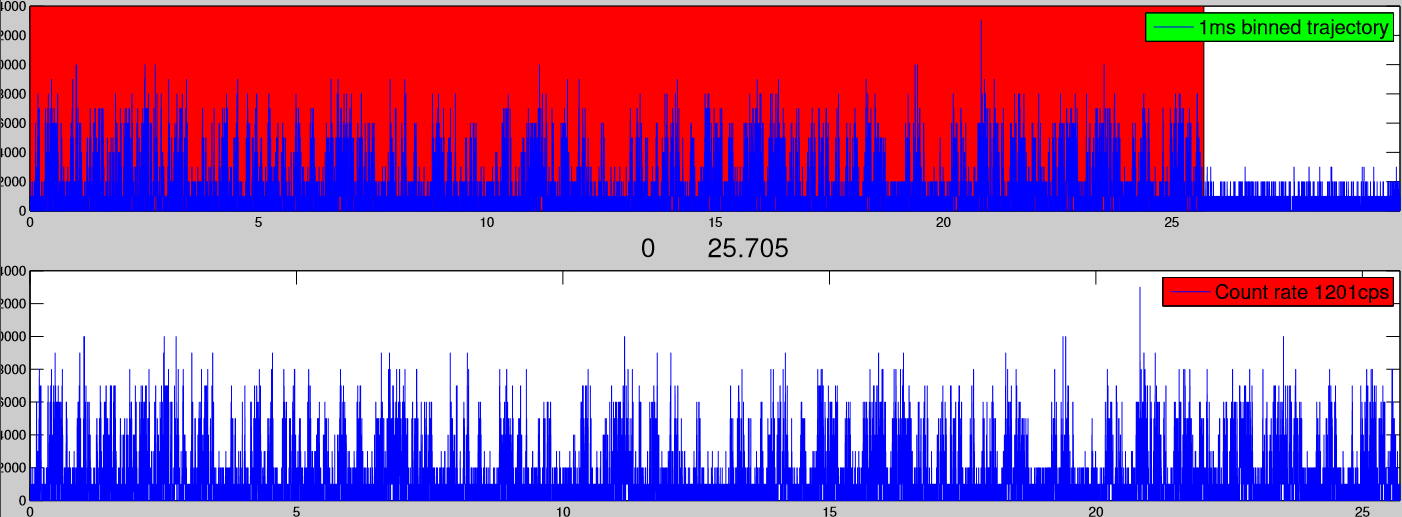
\includegraphics[width=\textwidth]{timetrace_selection}
\caption{Selection of a timetrace with a program written in MATLAB R2012b and C to select the parts of the timetrace (in red) that will be put into .dat files. As in this specific case the Cu-Azurin bleached around 25.7 second mark and the timetrace once it is bleached is not of interest and therefore not selected.}
\label{timetrace_selection}
\end{figure}

Once the timetrace is selected and put into several .dat files, another C program is run to precisely calculate the  on- ($\tau_{on}$) and off times ($\tau_{off}$). This program uses several mathematical methods to calculate the timestamps and intensity of intensity jumps in optical single molecule emission data that exhibit discrete intensity jumps, in detail described by Lucas P. Watkins and Haw Yang in their paper \cite{And2004}. As an example, several on- and off times are visualized in Figure \ref{on_off_times}. These times are defined as the duration of the CuAz being oxidized ($\tau_{on}$) and reduced ($\tau_{off}$). The intensity jumps that are controlled is what is referred to as 'switching' while the (often) unwanted and uncontrolled switching between the bright 'on' and dark 'off' states is called 'blinking'. 

\subsection*{Results and discussion timetraces CuAz}

Looking at the timetraces between 100mV and 0mV (Figure \ref{plots_timetraces_diff_pot}) a trend is noticeable on sight. For the higher potentials, the $\tau_{off}$ are long and the $\tau_{on}$ are relatively short which goes hand in hand with the low amount of events. When the potential decreases the amount of events start to increase and the $\tau_{on}$ becomes longer while $\tau_{off}$ becomes shorter. The explanation for this is simply the FluRedox principle. CuAz in oxidized form (copper is in $\textup{Cu}^{2+}$) shows an absorbence maximum around 628nm which overlaps with the fluorescence emission of the ATTO655 dye as is shown earlier in Figure \ref{}. Since FRET is high in this form, the fluorescence of the dye is quenched resulting in longer $\tau_{off}$. When the potential is decreasing, the solution is reducing. When CuAz is reduced - since the absorption at 628nm disappears upon reduction - the FRET is low and thus the dye  shows high fluorescence and longer $\tau_{on}$ times are expected. This principle seems to be the only role in play until the potential comes near 25mV. Here a new phenomenon is noticeable. Beside the expected  increasing $\tau_{on}$ and decreasing $\tau_{off}$ due to switching of CuAz, a secondary timescale seems to be shown in the form of very short $\tau_{on}$ in very short succession. To explain this event, a closer look has to be taken at the chemicals involved in the chemical processes concerning the redox reactions. Apart from the intramolecular electron transfer between the label and the copper center, intermolecular reactions between the redox active components in the solution and the dye are also present. Intermolecular reactions between the copper center and the solution are disregarded because of the longer time scale within which electron transfer occurs (is this true Bis?). 

\begin{figure}[ht!]
\centering
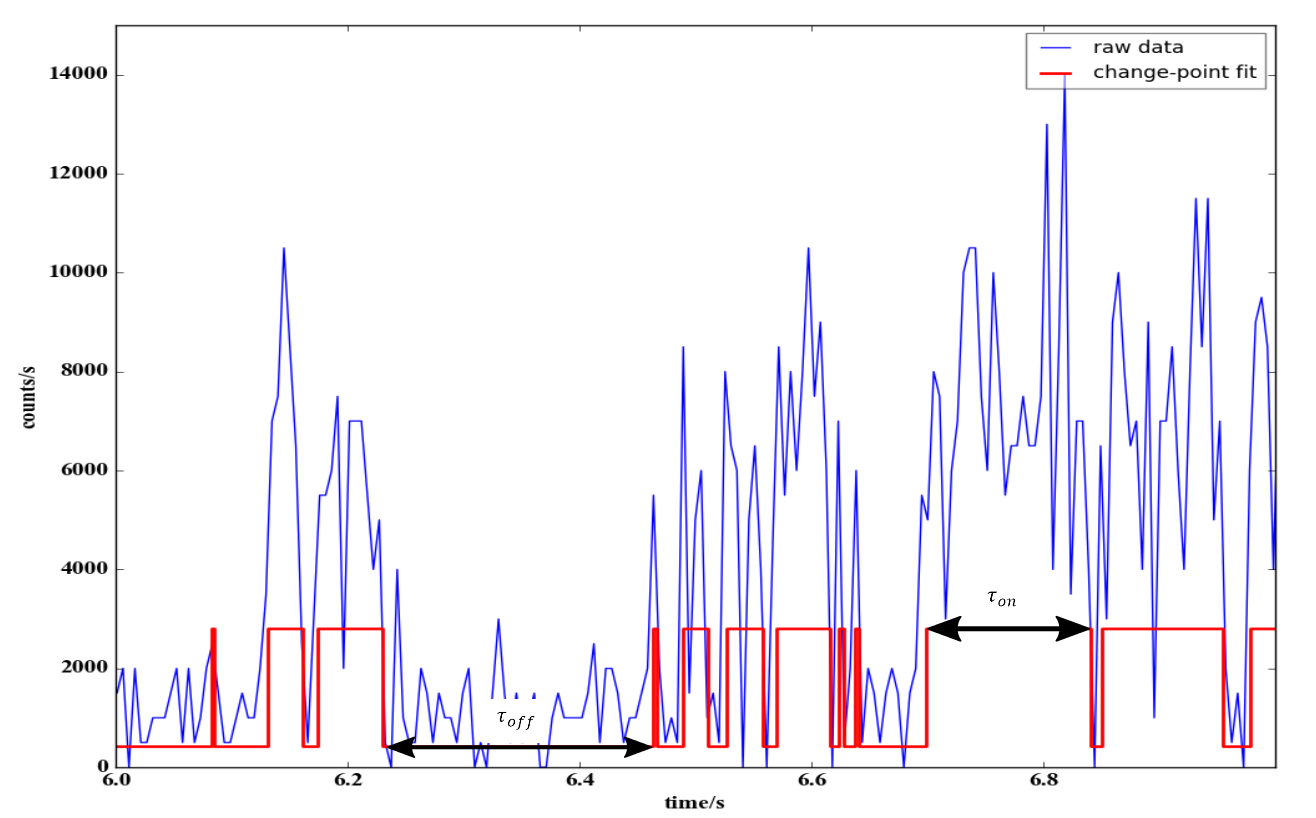
\includegraphics[width=\textwidth]{on_off_test1}
\caption{Same timetrace as Figure \ref{timetrace_selection} but a smaller range. In red is plotted the calculated intensity jumps according to the program written by Lucas P. Watkins and Haw Yang. The time when the intensity is low is refered to as the $\tau_{off}$ and the time the molecules intensity is high is the $\tau_{on}$.}
\label{on_off_times}
\end{figure}

\begin{figure}[ht!]
\centering
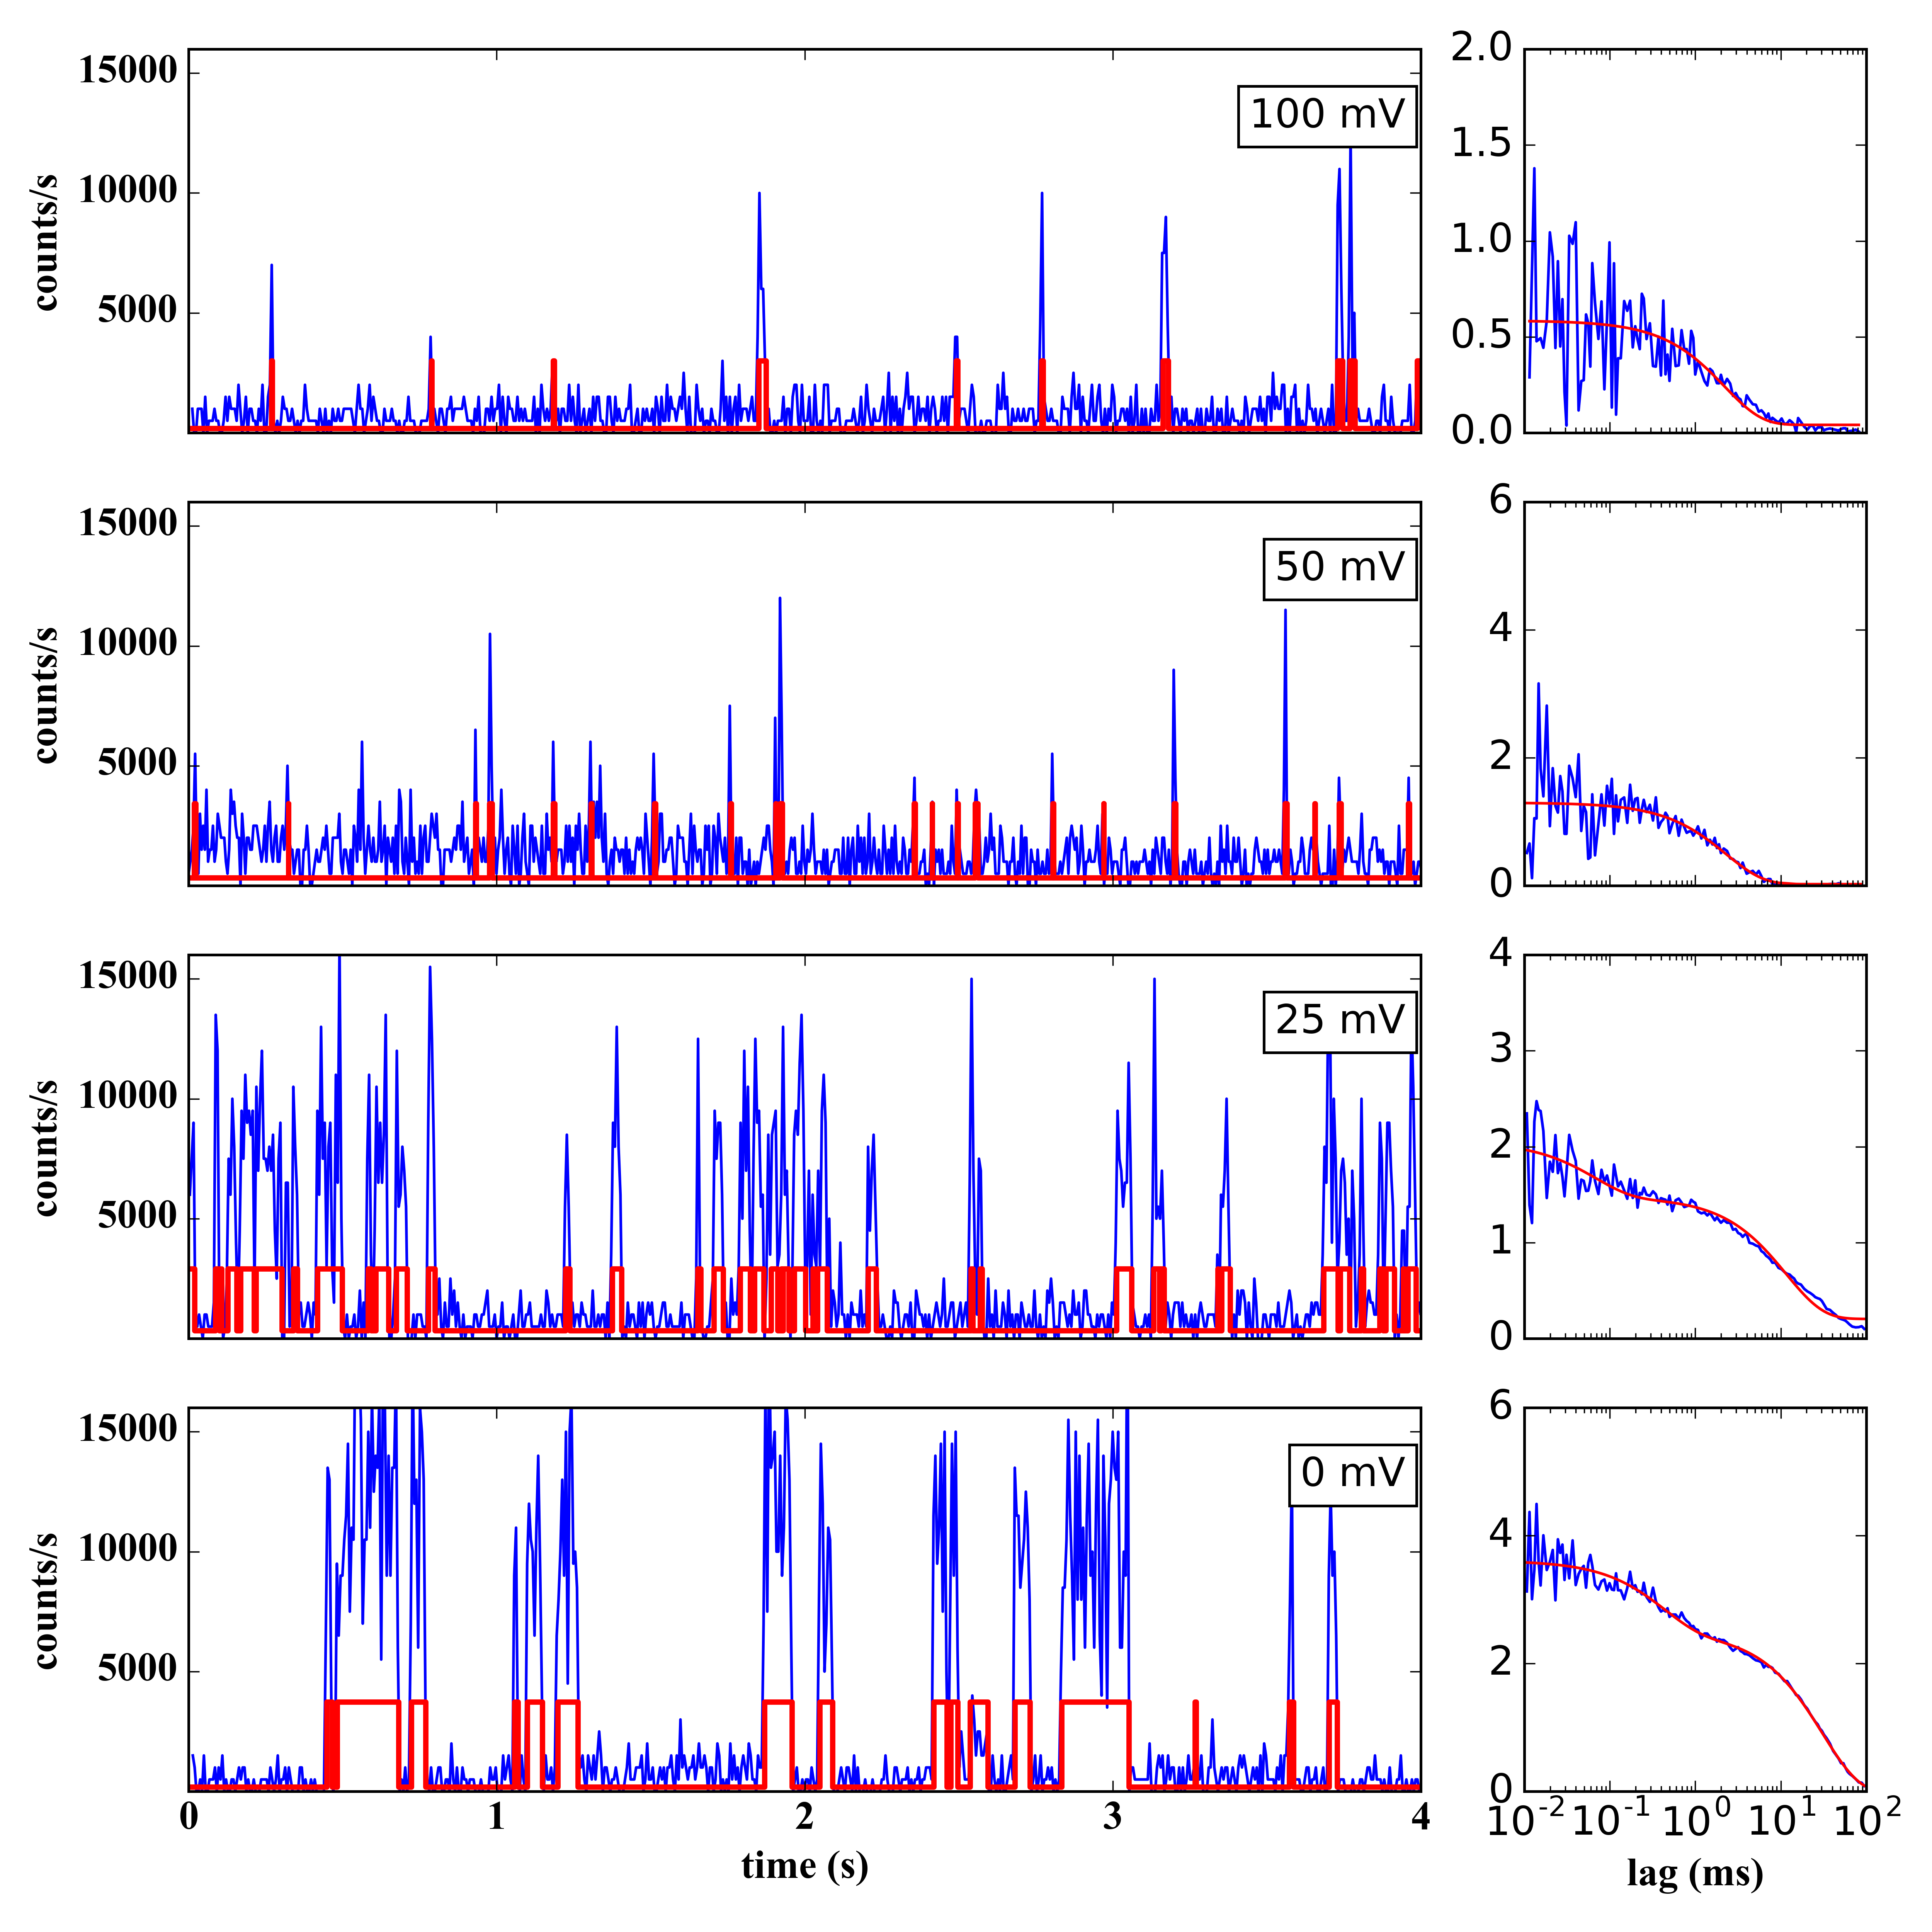
\includegraphics[width=1\textwidth]{plots_timetraces_diff_pot}
\caption{Timetraces of the same CuAz molecule under different potentials. A clear difference between $\tau_{on}$ and $\tau_{on}$ under different potentials is visible: shorter $\tau_{on}$ for higher oxidizing potentials, longer $\tau_{on}$ for reducing lower potentials. For potentials below 25mV this pattern gets disturbed due to blinking of the ATTO665.}
\label{plots_timetraces_diff_pot}
\end{figure}



\end{document}
